\RequirePackage{atbegshi}
\documentclass{beamer}

%\usepackage{beamerarticle}

\usepackage{beamerthemesplit}
\usepackage{graphicx}
\usepackage{xypic}
\usepackage{hyperref}
\usepackage{wrapfig}
\usepackage{color}

\title{A Radio Relay System for Remote Sensors in the Antarctic}
\subtitle{Final Seminar}
\author{Mark Jessop}
\date{October 8, 2010}

\pgfdeclareimage[height=1.3cm]{logo}{images/ualogo_spot.pdf} 

\usepackage[absolute,overlay]{textpos} 
\setlength{\TPHorizModule}{1mm} 
\setlength{\TPVertModule}{1mm} 
\newcommand{\MyLogo}{% 
\begin{textblock}{14}(104.0,0.3) 
  \pgfuseimage{logo} 
\end{textblock} 
} 

\definecolor{uofa}{cmyk}{1,0.56,0,0.18}
\usecolortheme[named=uofa]{structure}

\begin{document}

\frame{
\MyLogo
\titlepage
\begin{center}
%\small{Supervisor: Dr Chris Coleman}% \hspace{20pt} Co-Supervisor: Dr  Said Al-Sarawi}
\end{center}
}

%\section[Outline]{}
%\frame{\tableofcontents}

\section{Introduction}

\subsection{Motivation}
\frame{\MyLogo
\frametitle{Motivation}
\textbf{Aim} - Design and build a low power HF data transmitter for use in an antarctic remote sensor application.\\
\begin{itemize}
\item Project scope expanded mid-year to include other applications.
\item{Initial Constraints still used.\\ 
\begin{itemize}
\item Low Temperature Operation
\item Low Power Consumption
\end{itemize}
}

\item Can be used in a huge amount of applications!
\end{itemize}
}

\subsection{Hardware \& Software Overview}
\frame{\MyLogo
\frametitle{Hardware \& Software Overview}
\begin{itemize}
\item Modular Design \& Construction
\end{itemize}
}
\frame{\MyLogo
\frametitle{Hardware \& Software Overview}
\begin{figure}
  \begin{center}
    \includegraphics[width=1\textwidth]{diagrams/Antarctic_Radio_Overview.pdf}
  \end{center}

\end{figure}

}

\section{Hardware}

\subsection{CPU}
\frame{\MyLogo
\frametitle{CPU - Atmel ATXmega128A1}
\begin{figure}
  \begin{center}
    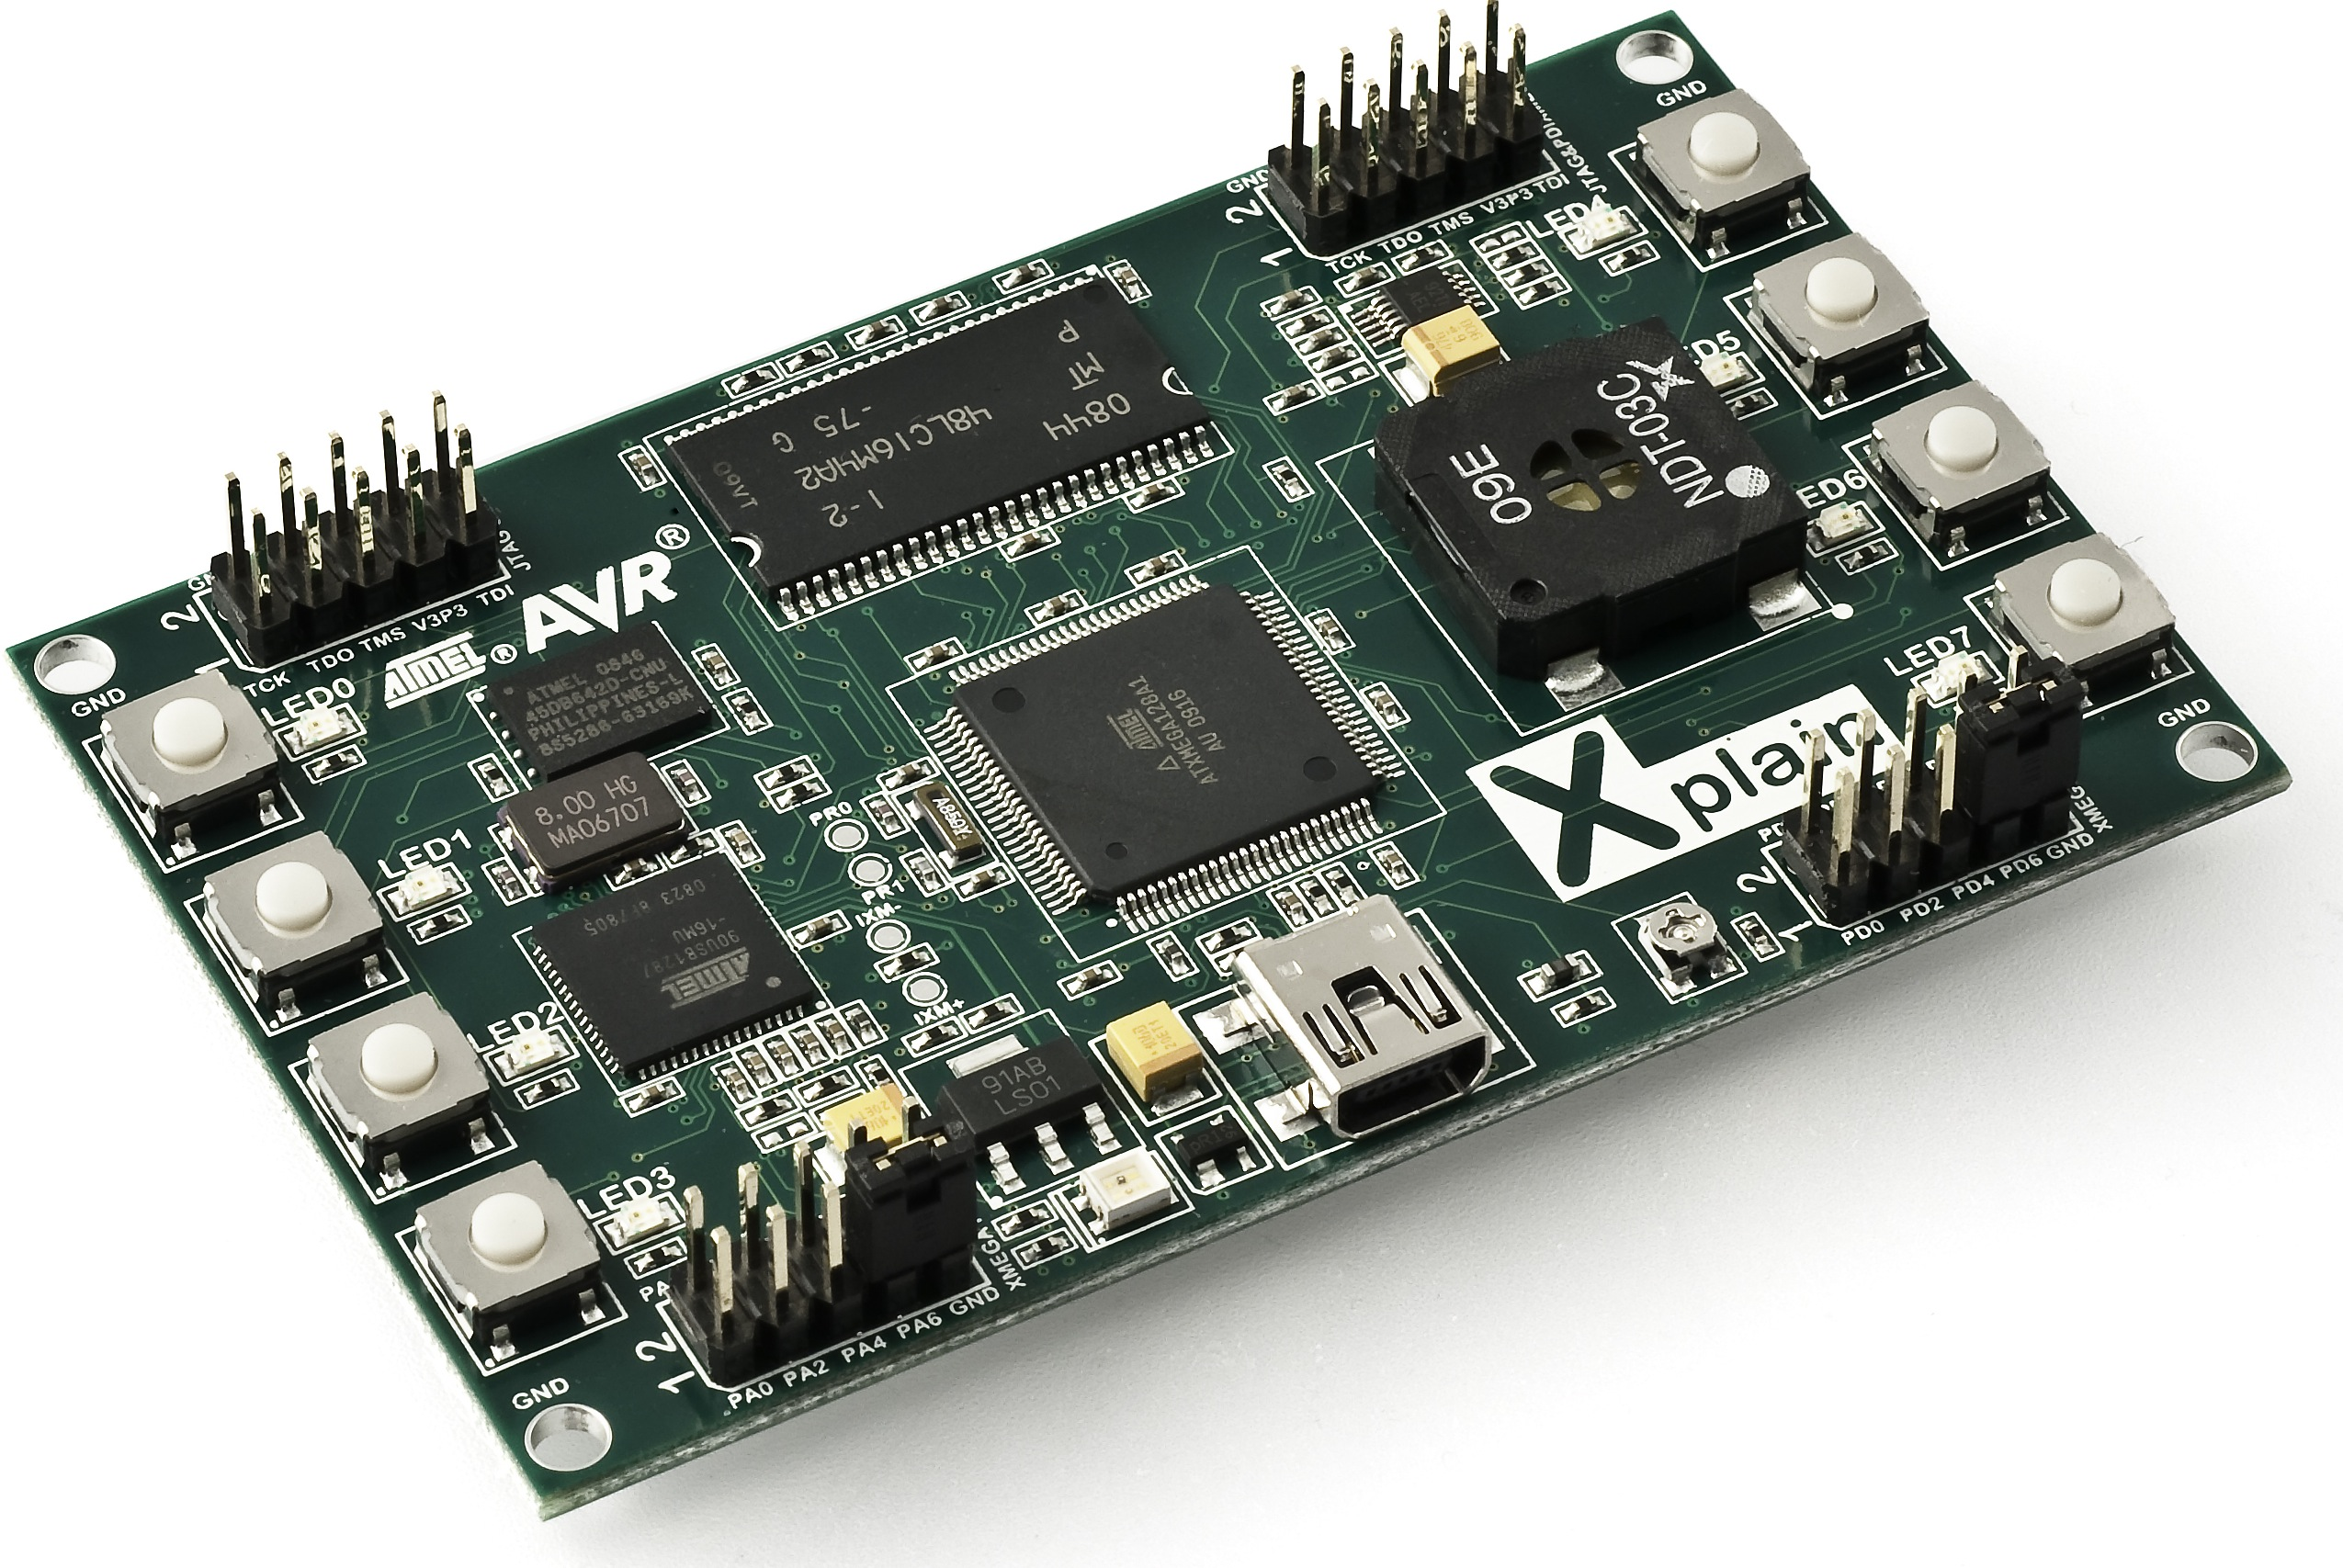
\includegraphics[width=0.4\textwidth]{images/xplain.jpg}
  \end{center}
  %\caption{Atmel XPlain Development Board}
  \label{xplain}
\end{figure}
\textbf{Atmel XPlain Development Board}
\begin{itemize}
\item Atmel ATXmega128A1 Micro-Controller, clocked at 32MHz
\item 8MB SDRAM
\item 8MB NAND Flash Memory
\item Low Power Consumption - 18mA @ 32MHz, 1.4mA @ 2MHz, $1.16\mu A$ Power-Save
\end{itemize}
}

\subsection{Signal Generator}
\frame{\MyLogo
\frametitle{Signal Generator - Analog Devices AD9835}
\begin{itemize}
\item Original intention was to use an AD9834
\item AD9835 Board ended up having the same power requirements!
\end{itemize}

\begin{figure}
  \begin{center}
    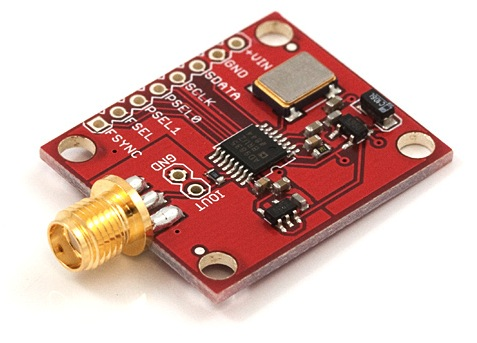
\includegraphics[width=0.25\textwidth]{images/ad9835.jpg}
  \end{center}
  %\caption{Atmel XPlain Development Board}
  \label{ad9835}
\end{figure}
\textbf{Analog Devices AD9835}
\begin{itemize}
\item Can generate Sine-waves between 1Hz - 25MHz.
\item 2 programmable (via SPI) frequency registers.
\item Dedicated pins for switching between registers.
\item Using 16MHz SPI clock, can reprogram at 7500Hz.
\end{itemize}
}

\subsection{Power Amplifier}
\frame{\MyLogo
\frametitle{Power Amplifier}
\begin{itemize}
\item Op-Amp based pre-amplifier - 40mW output.
\item Class C NPN Transistor Amplifier - 1W output.
\item Class E MOSFET Power Amplifier - 5W output.
\end{itemize}
}

\subsection{Power Supply}
\frame{\MyLogo
\frametitle{Power Supply}
\textbf{Supply Requirements}
\begin{itemize}
\item 12v, 5v and 3.3v rails are required.
\item Linear Regulators are very in-efficient.
\item Switch-mode Regulators used instead.
\end{itemize}
\textbf{Battery Power}
\begin{itemize}
\item Powered from a 12V SLA for testing.
\item For sub-zero use, Lithium-iron primary cells can be used.
\item Lithium-thionyl chloride secondary cells can operate down to $-60^\circ$C.
\end{itemize}
}

\subsection{Hardware Testing}

\frame{\MyLogo
\frametitle{Low Temperature Testing}
\begin{itemize}
\item All major components rated to either $-40^\circ$C or $-55^\circ$C.
\item Doesn't hurt to check!
\item Dry Ice used to cool components below rated limits.
\end{itemize}

\begin{figure}
  \begin{center}
    \includegraphics[width=0.6\textwidth]{images/cold_xmega.jpg}
  \end{center}
\end{figure}
}

\frame{\MyLogo
\frametitle{Low Temperature Testing}
\begin{figure}
  \begin{center}
    \includegraphics[width=0.6\textwidth]{images/cold_xmega2.jpg}
  \end{center}
\end{figure}
\begin{itemize}
\item AT-XMega's internal RC 32MHz oscillator drifts up to 33MHz at $-55^\circ$C.
\item AD9835's output only drifts up by $\sim$300Hz at $-40^\circ$C!
\end{itemize}
}

\section{Software}
\subsection{Overview}
\frame{\MyLogo
\frametitle{Software Overview}
\begin{itemize}
\item Coded in C and C++.
\item Libraries built first, more complex applications later.
\item Morse, RTTY (FSK) and DominoEX modulation implemented.
\item Data acquisition from onboard ADCs, UARTs, or I$^2$C Devices.
\end{itemize}
}

\subsection{Morse}
\frame{\MyLogo
\frametitle{Morse Code \& QRSS}

\begin{itemize}
\item Morse Code at very slow speeds can be received over very long distances.
\item Signals are pulled out of the noise floor with DSP techniques.
\item Very low signal bandwidth.
\item Not very useful for transmitting lots of data.
\item Good for beaconing.
\end{itemize}

\begin{figure}
  \begin{center}
    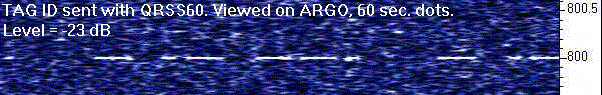
\includegraphics[width=0.8\textwidth]{images/tag60sec.png}
  \end{center}
  \caption{QRSS Morse Broadcast, signal level -23dB below the noise floor.}
  \label{qrss}
\end{figure}
}

\subsection{RTTY}
\frame{\MyLogo
\frametitle{RTTY (FSK)}
\begin{itemize}
\item FSK Modulation, with start and stop bits.
\item Implemented to operate between 50 and 300 baud (symbols/sec).
\item Carrier Shift programmable from 170 to 425Hz.
\item Plenty of existing software to decode RTTY (i.e. fldigi)
\end{itemize}

\begin{figure}
  \begin{center}
    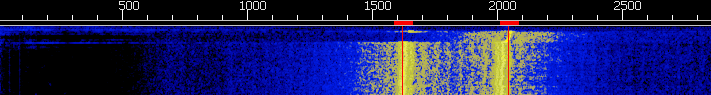
\includegraphics[width=0.8\textwidth]{images/rtty.png}
  \end{center}
  \caption{300 Baud RTTY, with 425Hz Carrier Shift}
  \label{rtty}
\end{figure}
}

\subsection{DominoEX}
\frame{\MyLogo
\frametitle{DominoEX (MFSK)}
\begin{itemize}
\item The first MFSK-based mode implemented - utilises Incremental Frequency Shift Keying.
\item Resistant to multi-path and doppler effects.
\item 6 variations available, each with different symbol rates (3.9 to 29.5Hz) and bandwidths (173 to 524Hz).
\item Data rates varying from 2 to 14 \emph{characters} per second.
\end{itemize}

\begin{figure}
  \begin{center}
    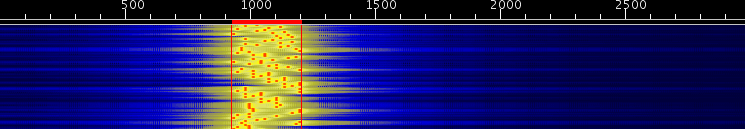
\includegraphics[width=0.8\textwidth]{images/dominoex.png}
  \end{center}
  \caption{DominoEX8 - 7.8125 baud, 346Hz Bandwidth }
  \label{domino}
\end{figure}
}

\subsection{Testing Procedures}
\frame{\MyLogo
\frametitle{Testing Procedures}

\begin{itemize}
\item Checking of library operation once coded.
\end{itemize}

}


\section{Example Application \& Prototype}
\frame{\MyLogo
\frametitle{Example Application - HAB Telemetry Transmitter}

\begin{columns}[c]
\column{7cm}
\textbf{Amateur High Altitude Ballooning (HAB)}
\begin{itemize}
\item Aims to set height / distance records for balloon flights.
\item Some form of telemetry system used to track balloon in flight.
\item 433MHz Single-Sideband Transmissions commonly used.
\end{itemize}

\column{3cm}
\begin{figure}
  \begin{center}
    \includegraphics[width=3cm]{images/horus_launch.jpg}
  \end{center}
\end{figure}

\end{columns}
}

\frame{\MyLogo
\frametitle{Example Application - HAB Telemetry Transmitter}
\begin{figure}
  \begin{center}
    \includegraphics[width=10cm]{images/horus_33km.jpg}
  \end{center}
\end{figure}
\begin{itemize}
\item Local Amateur HAB group - \textbf{Project Horus}
\item{Have offered to fly a prototype transmitter, with modifications.\\
\begin{itemize}
\item GPS Receiver, for positioning information
\item Temperature Sensors
\end{itemize}
}
\end{itemize}
}

\frame{\MyLogo
\frametitle{Prototype}
\begin{itemize}
\item{ System `Motherboard'\\
\begin{itemize}
\item XMega
\item AD9835 DDS VFO
\item UBlox5 GPS Module
\item I$^2$C Temperature Sensors
\end{itemize}}

\item Amplifier Module
\end{itemize}

}


\frame{\MyLogo
\frametitle{References}
\tiny{
Saft \textit{Lithium-thionyl chloride (Li-SOCl2) Cell Range}\\
\url{http://www.saftbatteries.com/Produit\_LSH\_cell\_range\_303\_8/Default.aspx}

}
}

\end{document}